% !TEX encoding = UTF-8
% !TEX TS-program = pdflatex
% !TEX root = ../tesi.tex

%**************************************************************
\chapter{Gestione documentale}
\label{cap:gestione-documentale}
%**************************************************************

\intro{Il seguente capitolo riporta una descrizione dettagliata del software F12 Documentale fornitomi per l'archiviazione dei documenti in upload durante la registrazione di un protocollo.\\
Nelle immagini esplicative i dati sensibili di aziende o persone sono oscurati per motivi di privacy.}\\

\section{F12 - Documentale}
Il software documentale sviluppato da Gestiware nasce per migliorare e potenziare il livello di integrazione fra F12 e una gestione documenale web esterna.

    \subsection{Tipologie di documenti}
    Di seguito le categorie di documenti che vengono gestite:
    \begin{itemize}
        \item documenti prodotti da F12 (flusso attivo);
        
        \item documenti da flusso passivo (flusso passivo);
        
        \item documenti tecnici o estemporanei collegati a varie entità di F12.
    \end{itemize}
    
    Ogni documento sarà associato ad un tipo di documento. Il tipo del documento identifica una classe di documenti (ad esempio le “fatture”) e quindi definisce lo schema di informazioni aggiuntive che hanno attinenza con i documenti così classificati. Queste informazioni di corredo verranno chiamati metadati. Ogni documento appartiene ad una ed una sola classe.
    \\
    \\
    È possibile creare una configurazione dove vengono definiti i tipi di documenti che vogliamo gestire (fattura, ddt,...,generico) e i metadati che vogliamo associare ad ogni tipo di documento. Per ogni metadato è possibile configurare il singolo campo di database dove il metadato può essere letto. Questo serve per poter estrarre o aggiornare i metadati di un documento automaticamente nel momento in cui questo viene caricato.
    \\
    \\
    Tutti i documenti di F12 avranno i seguenti metadati in comune:
    \begin{itemize}
        \item seriale;
        
        \item tipo\_documento;
        
        \item autore;
        
        \item data\_caricamento;
        
        \item data\_ultima\_modifica;
        
        \item barcode.
    \end{itemize}
    
    I documenti vengono identificati per mezzo di un seriale univoco che non permette la coesistenza, nel gestore documentale, di due documenti (semanticamente) distinti con lo stesso seriale. Ogni documento potrà avere anche un barcode associato.
    \\
    Inoltre può subire delle variazioni o essere modificato, questo comporta un aggiornamento della versione del documento. La nuova versione del documento ha lo stesso seriale ma ha incrementato il contatore della sua versione.
    
    \subsection{Flusso attivo}
    I documenti generati dal gestionale possono essere archiviati nel sistema documentale mediante due modalità:
    \begin{itemize}
        \item nel momento in cui F12 genera un nuovo documento, invoca una procedura del sistema documentale passandogli il file generato e i dati necessari all'archiviazione;
        
        \item la seconda modalità consiste in una procedura che elabora i file generati dalla coda di stampa e associa automaticamente il file all'entità corrispondente, basandosi sul nome del file oppure sull'xml associato al file contente i dati necessari all'archiviazione documentale.
    \end{itemize}
    
    \subsection{Flusso passivo}
    I documenti possono essere caricati manualmente attraverso l'interfaccia web presente sulle maschere di F12 oppure attraverso il portale web documentale.
    \\
    I documenti caricati tramite F12 sono collegati automaticamente all'entità di F12 in quanto il caricamento del file avviene sull'entità stessa.
    \\
    In caso di caricamento di file da portale web verranno richieste le informazioni necessarie al collegamento automatico del documento con l'entità di F12 (tipo entità, seriale, barcode ecc...).
    
    \subsection{Permessi su file e sicurezza}
    I permessi e le azioni che l'utente può effettuare sui file saranno ereditati dai permessi collegati ai gruppi di F12.
    \\
    È necessario aggiungere alla tabella di configurazione delle “tipologie dei documenti” un campo per settare il permesso corrispondete al gruppo per poter operare su quel tipo di documento.
    \\
    Ad esempio il gruppo amministrazione sarà associato ai documenti di tipo fattura.
    \\
    I file sono archiviati nel file system in forma criptata, senza estensione, di modo che siano leggibili solo attraverso il software documentale.

    \subsection{Gestione dei documenti}
    L'accesso al gestore documentale può essere effettuata sia lato web che lato client F12, e l'aggiunta di documenti alle entità di F12 potrà essere fatta da entrambi i lati.
        
        \subsubsection{Accesso documentale con F12}
        L'accesso all'interfaccia documentale su F12 avviene attraverso una maschera web caricata all'interno dell'entità per la quale si vuole abilitare il documentale e si potranno caricare documenti di tipologie abilitate per quel tipo di entità. 
        \\
        Si possono inoltre caricare anche documenti generici, tuttavia per questo tipo di documenti non sono definiti altri metadati oltre a quelli base.
        \begin{figure}[!h] 
            \centering 
            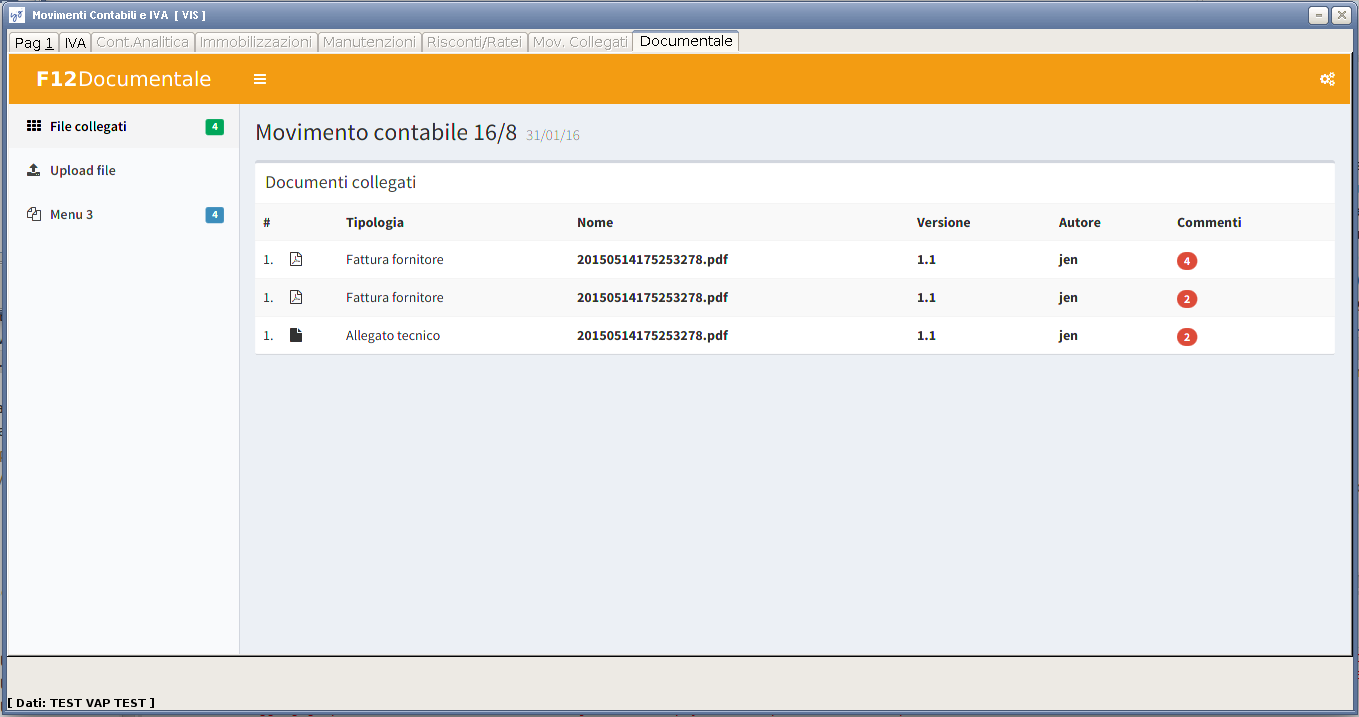
\includegraphics[width=1\columnwidth]{immagini/f12doc/1.png}
            \caption{Esempio di maschera documentale visibile per l'entità “movimento contabile 16/8”}
        \end{figure}
        \begin{figure}[!h] 
            \centering 
            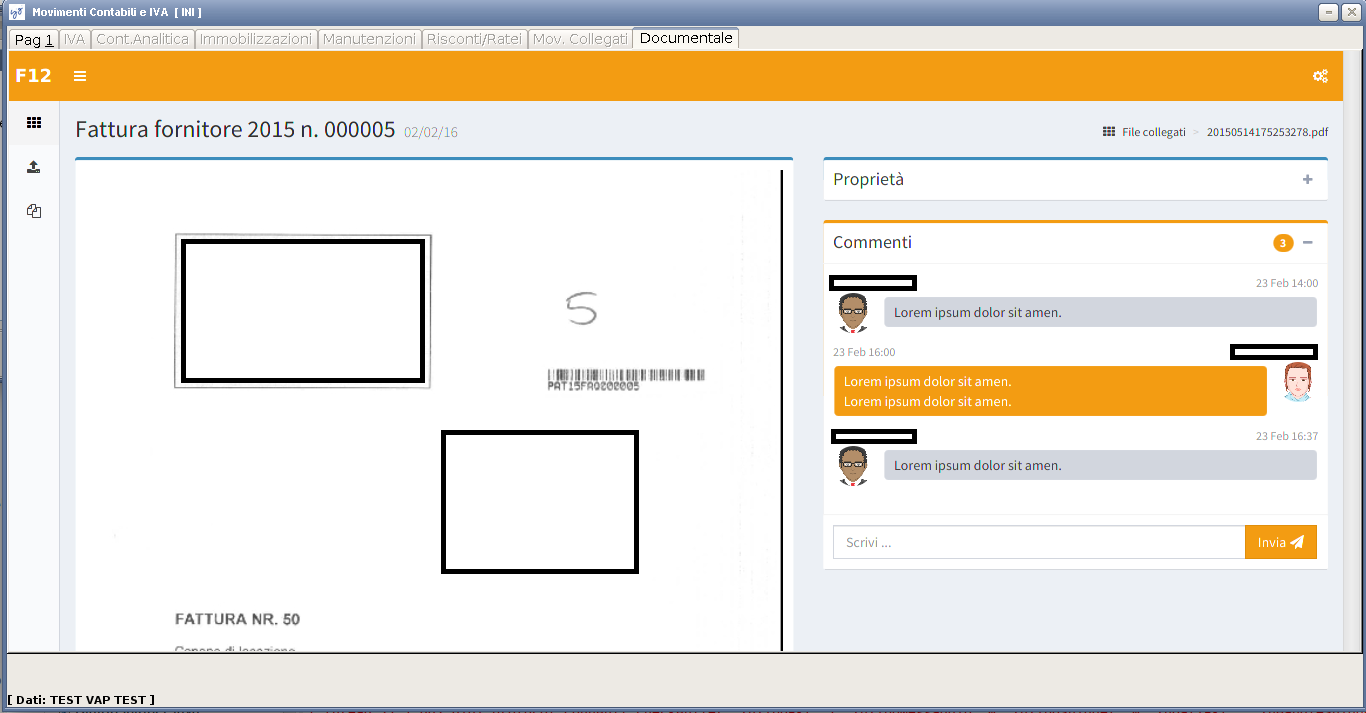
\includegraphics[width=1\columnwidth]{immagini/f12doc/2.png}
            \caption{Esempio di maschera di dettaglio di un documento 1}
        \end{figure}
        \begin{figure}[!h] 
            \centering 
            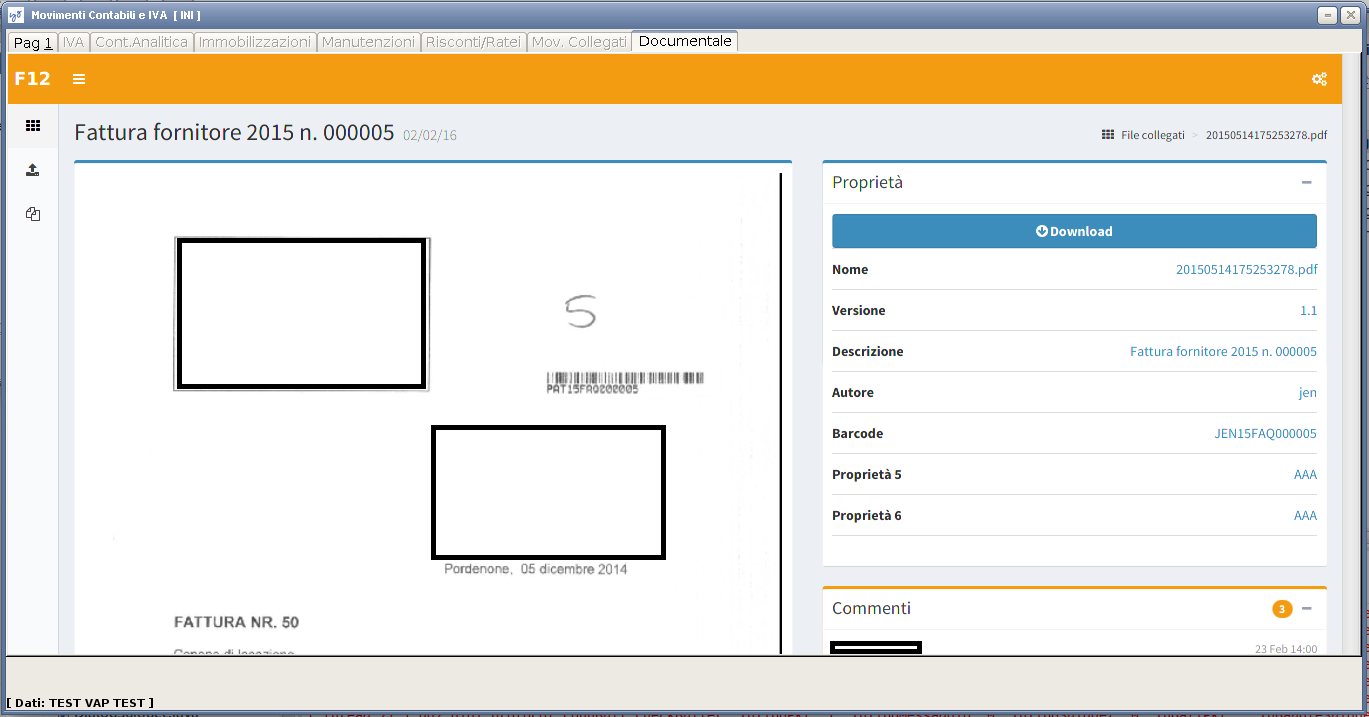
\includegraphics[width=1\columnwidth]{immagini/f12doc/3.png}
            \caption{Esempio di maschera di dettaglio di un documento 2}
        \end{figure}
        \newpage
        Attraverso questa maschera web si potranno:
        \begin{itemize}
            \item caricare documenti nuovi definendo preventivamente il tipo di documento che si sta caricando (Per aggiornare automaticamente i metadati);
            
            \item aggiungere, togliere, modificare metadati;
            
            \item caricare nuove versioni dello stesso documento;
            
            \item commentare i documenti.
        \end{itemize}
        È inoltre possibile ricercare e consultare i documenti su una maschera web caricata a parte.
        
        \subsubsection{Accesso documentale tramite Web}
        Sarà possibile accedere al documentale tramite interfaccia web.
        \\
        Attraverso essa si potranno:
        \begin{itemize}
            \item cercare documenti;
            
            \item sfogliare le directory della \textit{repository};
            
            \item consultare le anteprime dei documenti;
            
            \item scaricare i documenti;
            
            \item commentare  i documenti;
            
            \item aggiungere, togliere, modificare i metadati;
            
            \item gestire le tipologie di documenti e i metadati;
            
            \item caricare revisioni di un documento;
            
            \item caricare nuovi documenti attraverso un'apposita interfaccia (Si potranno stabilire delle condizioni attraverso le quali i nuovi documenti caricati saranno collegati automaticamente alle entità di F12).
        \end{itemize}
        \begin{figure}[!h] 
            \centering 
            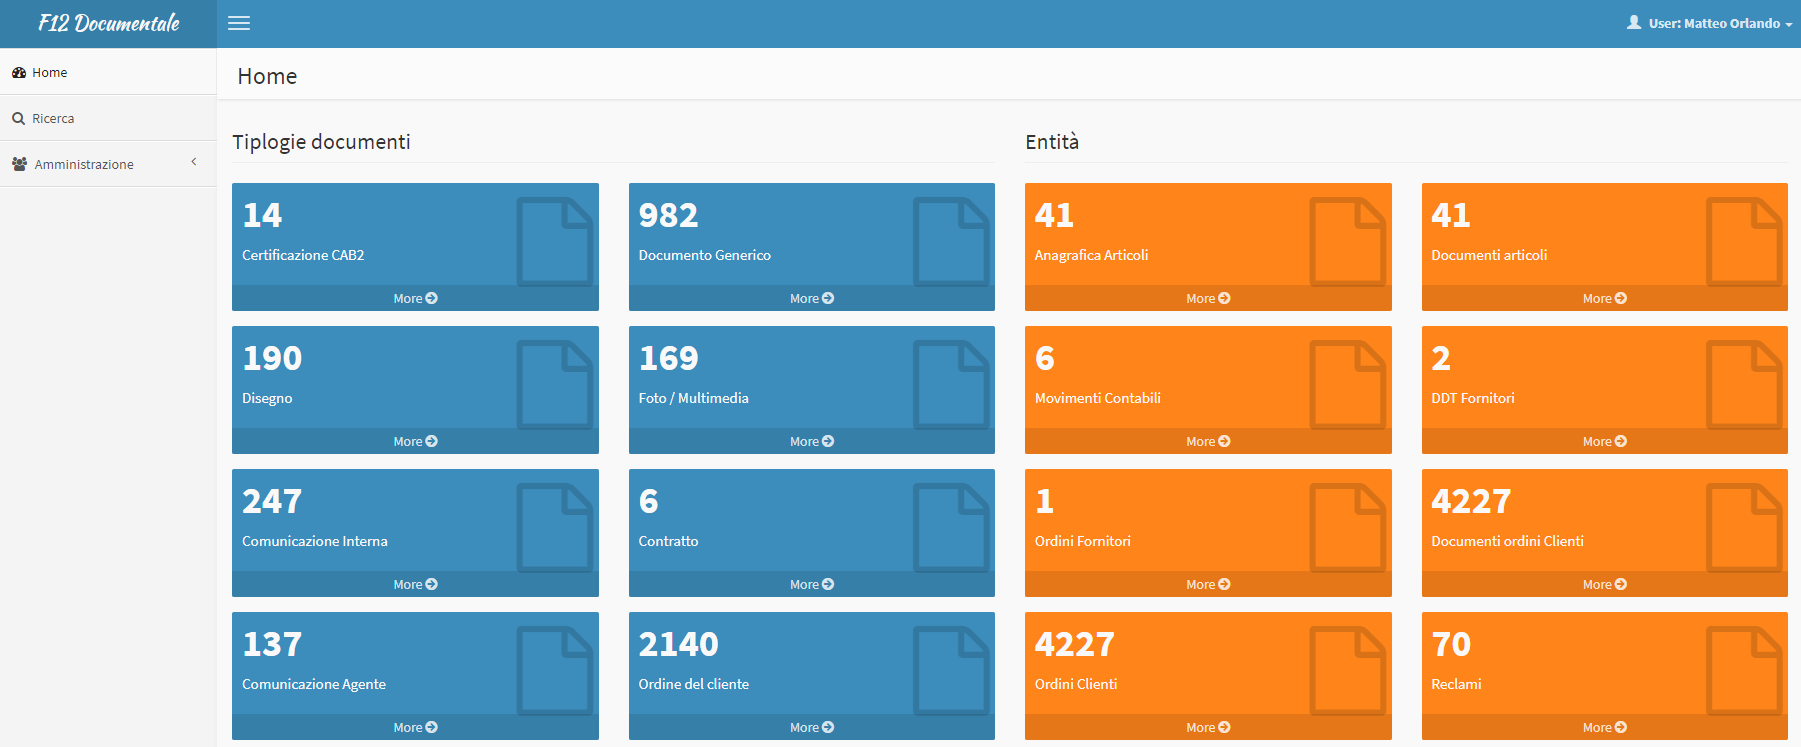
\includegraphics[width=1\columnwidth]{immagini/f12doc/4.png}
            \caption{Esempio di maschera documentale visibile per l'entità “movimento contabile 16/8”}
        \end{figure}